\documentclass[11pt,letterpaper]{article}
\usepackage[margin=1in]{geometry}
\usepackage{times}
\usepackage{microtype}
\usepackage{graphicx}
\usepackage{xcolor}
\usepackage{booktabs}
\usepackage{longtable}
\usepackage{array}
\usepackage{hyperref}
\hypersetup{colorlinks=true, urlcolor=blue, linkcolor=blue}
\usepackage{listings}
\usepackage{titlesec}
\usepackage{enumitem}
\usepackage{caption}
\captionsetup{font=small}
\usepackage{tikz}
\usetikzlibrary{shapes.geometric,arrows.meta,positioning,decorations.pathreplacing,backgrounds,fit,calc,patterns}
\usepackage{pgfplots}
\pgfplotsset{compat=1.18}

% Custom TikZ styles for the paper's figures
\tikzset{
  cdmbox/.style={draw, rounded corners=2pt, minimum height=0.8cm, font=\small, align=center},
  thinarrow/.style={-{Stealth[length=2mm,width=1.5mm]}, thick},
  fatarrow/.style={-{Stealth[length=3mm,width=2mm]}, very thick},
  layerbox/.style={draw, rounded corners=3pt, minimum height=1.4cm, minimum width=9cm, font=\small, align=left, inner sep=4pt},
  slotcell/.style={draw, minimum width=0.85cm, minimum height=0.7cm, font=\scriptsize, align=center, inner sep=2pt},
}

\lstset{
  basicstyle=\ttfamily\footnotesize,
  breaklines=true,
  frame=single,
  showstringspaces=false,
  numbers=left,
  numberstyle=\tiny\color{gray},
  numbersep=6pt
}

\title{\textbf{Anatomy of the Desktop DRM Stack:\\
A Three-Layer Dispatch Model in Widevine CDM\_11 and Its
Hardware-Decode Dormancy on Chrome}}

\author{
  Jeremy Erazo \textit{(\texttt{trexnegr0})} \\
  Independent security researcher \\
  \texttt{mendozayt13@gmail.com}
}

\date{Draft --- June 15, 2026}

\begin{document}
\maketitle

\begin{abstract}
\noindent
Widevine Content Decryption Module (CDM) ships in essentially every
major desktop browser and underlies the Encrypted Media Extensions
(EME) playback path for every major commercial streaming service.
The internals of the Windows L1 build are documented only
fragmentarily: header files describe the C++ ABI it presents to the
host browser, but the binary itself is closed source, partially
obfuscated, and behaves differently depending on whether the host
delegates decode to hardware-protected pipelines.
This paper presents a Buchanan-style architectural reverse engineering
of the CDM\_11 implementation as it ships in Chrome 149 and Edge 150
on Windows 11.  We identify a \emph{three-layer dispatch model} (outer
vtable thunks, an intermediate \texttt{m\_impl} vtable of clean
wrappers and double-trampolines, and per-slot handler bodies), we
locate each layer byte-by-byte in both binaries, and we empirically
characterise which slots are invoked during steady-state playback
versus which are dormant.  We runtime-confirm that during
hardware-decoded Netflix playback the user-facing per-frame slots of
the CDM\_11 interface (\texttt{Decrypt},
\texttt{DecryptAndDecodeFrame}, \texttt{DecryptAndDecodeSamples}) do
not fire while an internal singleton dispatch table generates
$\sim$2{,}300 calls per second of crypto / scheduler work that is
invisible from the EME boundary.  We document the distribution of
mixed-boolean-arithmetic style obfuscation across the slot space and
show that it is concentrated where the CDM begins to parse
attacker-controllable structured data, while remaining absent on slots
that pass opaque blobs.  We then verify reachability of the
session-management slots from two distinct EME applications (Netflix
and a public Widevine test source) and show identical dispatch
behaviour.  No content key, frame buffer, or ciphertext byte is
captured at any point in the study.
\end{abstract}

% =============================================================================
\section{Introduction}
\label{sec:intro}

Modern desktop video DRM is the bridge between commercial streaming
services and the browser's media pipeline.  When a user plays a video
in Netflix, Amazon Prime, Disney+ or any other Widevine-protected
source, the browser invokes Encrypted Media Extensions (EME) to
delegate the cryptographic operations to a Content Decryption Module
(CDM).  In Chromium-based browsers on Windows, that CDM is the
proprietary \texttt{widevinecdm.dll} library shipped by Google.
The browser loads the library inside a Mojo utility process
(\texttt{--utility-sub-type=media.mojom.\\CdmServiceBroker}), connects
to it over IPC, and asks the library to construct a CDM instance
implementing a stable C++ interface defined in
\texttt{content\_decryption\_module.h}.  From the host's point of view
the interface is small (nineteen virtual methods) and well documented:
\texttt{Initialize}, \texttt{GetStatusForPolicy},
\texttt{CreateSessionAndGenerateRequest},
\texttt{UpdateSession}, and twelve other methods that cover license
exchange, decryption, decode, and lifecycle.

From the \emph{library}'s point of view this clean nineteen-method
surface is the visible peak of a much larger iceberg.  The Windows L1
build of Widevine implements a multi-million-instruction obfuscated
runtime under tens of megabytes of closed source code, integrates
with Windows Protected Media Path (PMP) when hardware decode is
available, and is bound by a strict licensing regime that prohibits
study of its decryption internals.  Public knowledge of the
implementation is fragmentary.

The motivation for this study is methodological as much as it is
technical.  Several recent legal episodes have shown that
\emph{publishing what one learns} about DRM internals is more legally
exposed than \emph{learning it}, and that the reproducibility of a
result matters as much as the result itself.  Following the Buchanan
model of architectural reverse engineering --- probe everything,
document the technique, publish no extraction artefact --- we set out
to build a fully reproducible, fully open methodology for studying
the Widevine CDM and to apply it to the questions that are paper-able
without crossing the digital-rights-management circumvention line.

The contributions of this paper are:
\begin{enumerate}[itemsep=2pt,topsep=2pt]
  \item A \textbf{three-layer dispatch model} for CDM\_11 in modern
        Chromium-family widevinecdm.dll, byte-verified in two distinct
        browser builds (Chrome 149 and Edge 150).
  \item A \textbf{slot-by-slot reachability map} of the CDM\_11 outer
        vtable, runtime-confirmed against both Netflix HW-decoded
        playback and a non-Netflix public Widevine source (Bitmovin
        demo).
  \item An \textbf{empirical demonstration of hardware-decode
        dormancy} of the user-facing per-frame slots during
        steady-state playback, alongside the activity profile of an
        internal singleton dispatch table that handles work invisible
        from the EME boundary.
  \item A characterisation of the \textbf{obfuscation distribution}
        across CDM\_11 slots: MBA-style obfuscation appears at varying
        depths of the dispatch chain for slots that parse
        attacker-controllable structured input, and is absent from
        slots that pass opaque blobs.
  \item A \textbf{shape-only observation methodology} that captures
        per-slot dispatch metadata without ever reading content
        bytes, content keys, or initialisation-vector bytes from
        memory.  The full source for the methodology is released; no
        capture rig, frame dump, or weaponisable artefact is.
\end{enumerate}

Figure~\ref{fig:system-overview} sketches the end-to-end stack
under analysis: a host browser process delegates EME operations
through Mojo IPC to a Chromium utility process whose sole job is to
load \texttt{widevinecdm.dll}, construct a CDM instance via the
\texttt{CreateCdmInstance} export, and expose the nineteen-method
CDM\_11 interface back to the host through that same Mojo channel.

\begin{figure}[t]
\centering
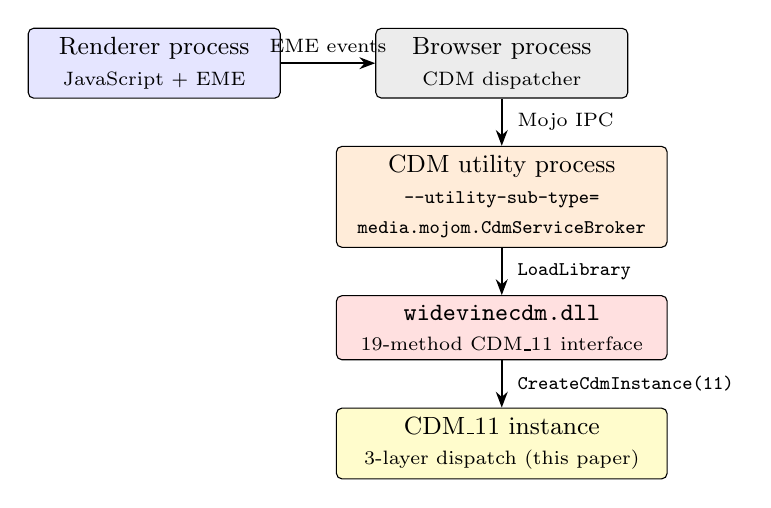
\begin{tikzpicture}[node distance=0.6cm and 1.2cm]
  \node[cdmbox, fill=blue!10, minimum width=3.2cm] (renderer) {Renderer process\\\scriptsize JavaScript + EME};
  \node[cdmbox, fill=gray!15, right=of renderer, minimum width=3.2cm] (browser) {Browser process\\\scriptsize CDM dispatcher};
  \node[cdmbox, fill=orange!15, below=of browser, minimum width=4.2cm] (utility) {CDM utility process\\\scriptsize \texttt{--utility-sub-type=}\\\scriptsize \texttt{media.mojom.CdmServiceBroker}};
  \node[cdmbox, fill=red!12, below=of utility, minimum width=4.2cm] (wvdll) {\texttt{widevinecdm.dll}\\\scriptsize 19-method CDM\_11 interface};
  \node[cdmbox, fill=yellow!20, below=of wvdll, minimum width=4.2cm] (cdmobj) {CDM\_11 instance\\\scriptsize 3-layer dispatch (this paper)};

  \draw[thinarrow] (renderer) -- node[above,font=\scriptsize] {EME events} (browser);
  \draw[thinarrow] (browser.south) -- node[right,font=\scriptsize,xshift=2pt] {Mojo IPC} (utility.north);
  \draw[thinarrow] (utility) -- node[right,font=\scriptsize,xshift=2pt] {\texttt{LoadLibrary}} (wvdll);
  \draw[thinarrow] (wvdll) -- node[right,font=\scriptsize,xshift=2pt] {\texttt{CreateCdmInstance(11)}} (cdmobj);
\end{tikzpicture}
\caption{End-to-end Widevine EME dispatch on Chromium-family browsers
on Windows.  The host browser delegates Encrypted Media Extensions
operations through Mojo IPC to a utility process whose sole purpose is
to load \texttt{widevinecdm.dll} and expose its CDM\_11 interface.
This paper studies the dispatch model that sits between the
\texttt{CreateCdmInstance}-returned interface and the per-slot
handlers inside the library.}
\label{fig:system-overview}
\end{figure}

The paper proceeds as follows.  Section~\ref{sec:background}
introduces the Widevine licensing levels, the EME dispatch path, and
the Windows PMP boundary.  Section~\ref{sec:threat} states the threat
model and ethical scope.  Section~\ref{sec:static} walks through the
static reverse engineering of the CDM\_11 dispatch.
Section~\ref{sec:runtime} describes the runtime instrumentation.
Section~\ref{sec:findings} presents the empirical findings.
Section~\ref{sec:obfuscation} treats the obfuscation distribution as
its own architectural defence.
Section~\ref{sec:cross} establishes cross-binary and cross-source
stability.  Section~\ref{sec:robustness} reports on the
falsification tests that were run before publishing any claim.
Section~\ref{sec:related} situates the work in the existing
literature.  Section~\ref{sec:ethics} states what was not done and
why.  Section~\ref{sec:conclusion} concludes.

% =============================================================================
\section{Background}
\label{sec:background}

\subsection{Widevine Levels}

Widevine defines three security levels, denoted L1 through L3.

\textbf{L3} is a software-only implementation.  The cryptographic
state of the CDM is held in process memory inside an obfuscated
runtime.  Content keys are unwrapped by a whitebox-style cryptographic
core and applied to ciphertext segments in user-space buffers, and the
decrypted output is returned to the host through standard memory.
L3 streams typically top out at 480p or 540p; the licence terms
restrict content owners from releasing high-value catalogue at L3.

\textbf{L2} is a software CDM that holds at least its sensitive
operations behind a hardware-backed TEE on the host.  L2 sees limited
deployment on desktop.

\textbf{L1} is the desktop variant of interest in this paper.  Under
L1 the CDM cooperates with a platform protected-media pipeline (on
Windows: Protected Media Path with Output Protection Management, PMP /
OPM) so that the decrypted frames are never visible to user-space
code in the host browser.  The CDM still runs as a userspace utility
process, but the per-frame ciphertext is routed to a kernel- or
hardware-resident decoder whose output buffer is rendered directly to
a protected GPU surface.  4K streams from Netflix, Disney+, and
others typically require L1.

\subsection{The EME Dispatch Path}

A browser playing protected content speaks W3C Encrypted Media
Extensions to the JavaScript application.  The application provides
the encrypted media (an ISO-BMFF or DASH stream containing Common
Encryption boxes), supplies a Key System name
(\texttt{com.widevine.\\alpha}), and listens for a sequence of EME
events: \texttt{encrypted}, \texttt{message},
\texttt{keystatuseschange}.

Internally, Chromium routes EME events to the CDM dispatcher in the
browser process, which Mojo-RPCs them to the CDM utility.  Inside the
utility, \texttt{widevinecdm.dll}'s \texttt{CreateCdmInstance} export
constructs a versioned implementation of the CDM C++ interface
defined in
\texttt{media/cdm/api/content\_decryption\_module.h}\footnote{See
the Chromium source tree at \href{https://chromium.googlesource.com/}{chromium.googlesource.com}.}
The current interface version is CDM\_11; previous versions (CDM\_10,
CDM\_9, \dots) are preserved for compatibility and may be present in
the same binary.  Each version exposes nineteen virtual methods,
typically presented in the order:

\begin{lstlisting}[basicstyle=\ttfamily\scriptsize]
 0: Initialize
 1: GetStatusForPolicy
 2: SetServerCertificate
 3: CreateSessionAndGenerateRequest
 4: LoadSession
 5: UpdateSession
 6: CloseSession
 7: RemoveSession
 8: TimerExpired
 9: Decrypt
10: InitializeAudioDecoder
11: InitializeVideoDecoder
12: DeinitializeDecoder
13: ResetDecoder
14: DecryptAndDecodeFrame
15: DecryptAndDecodeSamples
16: OnPlatformChallengeResponse
17: OnQueryOutputProtectionStatus
18: OnStorageId
\end{lstlisting}

This nineteen-slot interface is the only formal contract between the
host browser and the CDM library.  Everything below it --- including
how a single \texttt{DecryptAndDecodeFrame} call eventually causes a
single frame of decoded video to land in a protected surface --- is
implementation detail.

\subsection{Hardware Decode and PMP}

On Windows~10 and Windows~11 with HEVC- or AV1-capable GPUs and an
appropriate Microsoft PlayReady / Widevine cooperative stack, the
browser can request that a stream be hardware-decoded into a
protected surface.  At the high level, this exchange runs as follows:

\begin{enumerate}[itemsep=2pt,topsep=2pt]
  \item Browser negotiates hardware-secure decryption as a
        \texttt{capabilities} attribute on the EME
        \texttt{MediaKeySystemConfiguration}.
  \item CDM acknowledges hardware capability.
  \item Per-frame ciphertext is delivered \emph{not} through the CDM's
        \texttt{Decrypt} or \texttt{DecryptAndDecodeFrame} slots, but
        through a kernel-protected pipeline involving
        \texttt{Media Foundation} Decryption / Decoder pipelines and
        the PMP user-mode component (\texttt{peauth.sys},
        \texttt{audioses.dll}, etc.).
  \item The decoded frame is rendered directly to a protected GPU
        surface that the host browser cannot read back through normal
        Direct3D APIs.
\end{enumerate}

A key consequence, which we confirm empirically below, is that under
L1 hardware decode the CDM\_11 user-facing surface does \emph{not}
participate in per-frame decryption.  Despite the interface having a
slot called \texttt{DecryptAndDecodeFrame}, that slot is not invoked
during steady-state playback.  The CDM does still participate in
session and license management, so its session-creation and
license-update slots remain reachable.

% =============================================================================
\section{Threat Model and Methodology}
\label{sec:threat}

\subsection{Threat Model}

We consider an honest user of a Chromium-family browser playing
hardware-decoded Widevine-protected content on Windows~11.  The user
has consented to research-grade instrumentation of their own browser
and has installed our reverse-engineering tools on their own
laboratory machine.  The browser executable is unmodified and signed
by the vendor.  The Widevine CDM is the vendor-shipped
\texttt{widevinecdm.dll} of the installed browser version.

We deliberately exclude from this study any threat model in which an
attacker captures decrypted frames.  Our concern is not the
exploitation potential of the CDM but its architectural shape and the
attack surface it presents to the host browser.

\subsection{Methodology}

We follow what we describe as the \emph{Buchanan model} of DRM
research: probe everything, document the technique, publish no
extraction artefact.

Concretely, our methodology has four invariants:

\begin{enumerate}[itemsep=2pt,topsep=2pt]
  \item \textbf{Shape-only observation.}  Any runtime hook we install
        is permitted to log dispatch metadata --- slot number,
        timestamp, register value hashes, structure-size fields ---
        but is forbidden from copying any pointer-target bytes
        belonging to ciphertext, decrypted frames, content key
        material, or initialisation vectors into any persistent
        storage or any out-of-process channel.
  \item \textbf{Provable absence.}  After every experiment we
        forensically verify that the storage produced is pure ASCII
        JSON consisting only of the permitted metadata fields and
        contains no binary blobs, no decoded content, and no key
        material.
  \item \textbf{Reversible mutation.}  All runtime modifications to
        the target process (vtable patches, hook installations, CFG
        bitmap registrations) are reversible, and we restore the
        target to its original state before publishing.
  \item \textbf{No content circumvention surface.}  We use the
        operator's own browser session to a commercial streaming
        service to confirm what the CDM does during steady state, but
        we never instrument the decoder, the kernel-side PMP
        component, the protected surface, or any other component
        positioned to materialise a decrypted frame.
\end{enumerate}

A natural-language consequence of these invariants is that our results
characterise the CDM's \emph{dispatch behaviour}, not its
\emph{cryptographic state}.  We can report how often a slot fires
during real playback, what register-tuple distribution it sees, what
the shape of its incoming buffer descriptor is.  We cannot and do not
report any byte of decoded content.

% =============================================================================
\section{Static Reverse Engineering of CDM\_11}
\label{sec:static}

This section walks through the static reverse engineering of the
CDM\_11 dispatch in \texttt{widevinecdm.dll}, in the order that we
performed it.  Two binaries were analysed in parallel:
\textbf{Chrome~149.0.7827.115}'s
\texttt{Application/149.0.7827.115/WidevineCdm/\_platform\_specific/win\_x64/widevinecdm.dll}
($\sim$22~MB), and the same library as it ships in
\textbf{Microsoft Edge~150} ($\sim$19~MB).  All RVAs are with respect
to the binary's image base.

\subsection{Step 1: \texttt{CreateCdmInstance} and the version
            switch}
\label{sec:static-export}

\texttt{CreateCdmInstance} is the only relevant export.  Parsing the
PE export table:

\begin{lstlisting}[basicstyle=\ttfamily\scriptsize]
Edge 150     CreateCdmInstance @ rva 0x1d0850
Chrome 149   CreateCdmInstance @ rva 0x1d2e10
\end{lstlisting}

Disassembling either entry shows a chain of small wrapper functions
that load a version word into \texttt{ecx} (CDM interface version
9, 10, or 11) and call a per-version constructor.  Naively scanning
the first \texttt{call} after each \texttt{mov ecx, 0xb} returns the
runtime's stack-check probe rather than the actual constructor.  A
robust discoverer (\texttt{cdm\_arch\_discover.py} in the released
methodology) instead enumerates all call targets reachable from
\texttt{CreateCdmInstance}, filters out callees that appear more than
twice (a structural heuristic for runtime helpers), and validates
each candidate by checking whether its body contains a sequence of
the form
\begin{lstlisting}[basicstyle=\ttfamily\scriptsize]
  lea reg, [rip + N]      ; load a candidate vtable RVA
  mov qword ptr [r?], reg ; install it at offset 0 of `this`
\end{lstlisting}

\noindent and whether the loaded RVA points into \texttt{.rdata} at a
location whose first nineteen QWORDs are all valid code pointers into
\texttt{.text}.  The first such candidate is reported as the CDM
constructor and the loaded RVA as its outer vtable.

\subsection{Step 2: Co-shipped CDM versions}
\label{sec:static-versions}

A subsequent \emph{exhaustive} scan of \texttt{.rdata} for
nineteen-slot structures matching the CDM thunk pattern (described
below) reveals \textbf{two} such structures per binary, spaced
\texttt{0xc0} bytes apart:

\begin{center}\small
\begin{tabular}{lcc}
\toprule
\textbf{Binary} & \textbf{vtable A} & \textbf{vtable B} \\
\midrule
Edge 150    & \texttt{0x780190} & \texttt{0x780250} \\
Chrome 149  & \texttt{0x768ee0} & \texttt{0x768fa0} \\
\bottomrule
\end{tabular}
\end{center}

Within each binary, both vtables share their per-frame decrypt entry
(slot 14 points to the same function in both A and B), but their
\texttt{Initialize} entries differ.  This is consistent with the
binary shipping both CDM\_10 and CDM\_11 vtables in support of host
browsers that have not yet upgraded to the newer interface, and is
in line with the Chromium header history.  In what follows we
identify \emph{vtable B} as the CDM\_11 outer vtable, since runtime
patches at \emph{vtable B}'s slot positions are observed to intercept
the EME-host-facing dispatch (Section~\ref{sec:runtime}).

\subsection{Step 3: The outer vtable thunk pattern}
\label{sec:static-thunk}

The outer vtable contains nineteen entries.  Most of them are
\emph{thunks} of the form:

\begin{lstlisting}[basicstyle=\ttfamily\scriptsize]
slot N thunk:
  mov rcx, qword ptr [rcx + 8]       ; this->m_impl
  mov rax, qword ptr [rcx]           ; m_impl->m_vtable
  mov rax, qword ptr [rax + 8*N]     ; slot N of m_impl_vtable
  mov rdx, qword ptr [rip + cfg_disp]; CFG dispatcher pointer
  jmp rdx                             ; CFG-protected tail-call
\end{lstlisting}

Each thunk is twenty-eight bytes followed by \texttt{int3} padding,
laid out in a uniform \texttt{0x20}-spaced sequence in \texttt{.text}
for slots 3 through 17.  We disassembled each thunk in both binaries
and confirmed the slot-index check (the offset in
\texttt{[rax + 8*N]} equals the slot number times eight) for fifteen
of fifteen thunked slots in each binary.

Slots 0 (\texttt{Initialize}), 1 (\texttt{GetStatusForPolicy}), and
18 (\texttt{OnStorageId}) are \emph{not} thunks; they are direct
implementations placed in \texttt{.text} at non-contiguous addresses.
Slot 2 (\texttt{SetServerCertificate}) is a thunk in both binaries
but dispatches via \texttt{[rax + 8]} rather than
\texttt{[rax + 0x10]} --- it shares an implementation with slot 1 at
the \texttt{m\_impl} layer.

\subsection{Step 4: The \texttt{m\_impl} vtable}
\label{sec:static-mimpl}

The outer thunk dispatches into an \emph{intermediate} vtable owned by
the \texttt{m\_impl} object that the outer class holds in
\texttt{this->m\_impl} (\texttt{[outer + 8]}).  Locating this
intermediate vtable in \texttt{.rdata} is the second step of the
static analysis.

We use a knownsignature pivot: the implementation of slot 5
(\texttt{UpdateSession}) was previously identified by examining the
external call-chain trace in
\texttt{research-notes/10-phase2-updatesession-call-chain.md}.  Its
inner wrapper sits at RVA \texttt{0x1d4ab0} in Edge 150.  Reverse-searching
\texttt{.rdata} for the QWORD value \texttt{image\_base + 0x1d4ab0}
yields a single occurrence; backing up five eight-byte entries gives
the address of the \texttt{m\_impl} vtable: RVA \texttt{0x77d370} in
Edge 150.  All nineteen surrounding QWORDs point into \texttt{.text},
confirming the candidate.

The Chrome 149 \texttt{m\_impl} vtable was located by the same
technique but is omitted here for brevity.

\subsection{Step 5: The \texttt{m\_impl} layer structure}
\label{sec:static-layer2}

Disassembling each entry of the \texttt{m\_impl} vtable reveals a
mixture of three body types:

\begin{enumerate}[itemsep=2pt,topsep=2pt]
  \item \textbf{Clean MSVC wrappers} (slots 2, 3, 4, 5, 6, 7, 18).
        These have a standard prologue (multiple
        \texttt{push}~callee-saves, \texttt{sub rsp, N}, stack canary
        load), allocate or borrow input copies, perform sanitisation,
        and then call into a deeper handler.  These are the slots
        that ingest variable-length attacker-influenced data
        (session-id strings, response payloads, init-data buffers).
  \item \textbf{Double-trampolines} (slots 0, 1, 8, 9, 11--17).
        Two-instruction bodies of the form
        \texttt{mov rcx, [rcx + N]} followed by \texttt{jmp <addr>}
        which forward the call to a deeper-layer handler without
        intermediate processing.
  \item \textbf{Stubs} (slot 10).  A two-instruction body
        \texttt{mov eax, 3 ; ret} that returns a constant error code
        without any further work.
\end{enumerate}

\noindent The \texttt{m\_impl} vtable, in other words, is mostly a
\emph{routing} layer; the actual work happens one indirection
further.

\subsection{Step 6: The three-layer dispatch model}
\label{sec:static-3layer}

Composing the previous five steps, the dispatch chain from a host
virtual call to a per-slot handler is:

\begin{center}
\small
\begin{tabular}{ll}
\textbf{Layer 1} & \texttt{outer\_vtable} (CDM\_11 public interface) \\
                 & \quad direct impl OR thunk to \texttt{m\_impl} \\
\textbf{Layer 2} & \texttt{m\_impl\_vtable} (intermediate routing) \\
                 & \quad clean wrappers, double-trampolines, stubs \\
\textbf{Layer 3} & per-slot handlers \\
                 & \quad scattered, mixed clean / obfuscated \\
\end{tabular}
\end{center}

\noindent Figure~\ref{fig:3layer} sketches the model.  Each public
virtual call traverses three indirections before reaching the
function that performs work.

\begin{figure}[h]
\centering
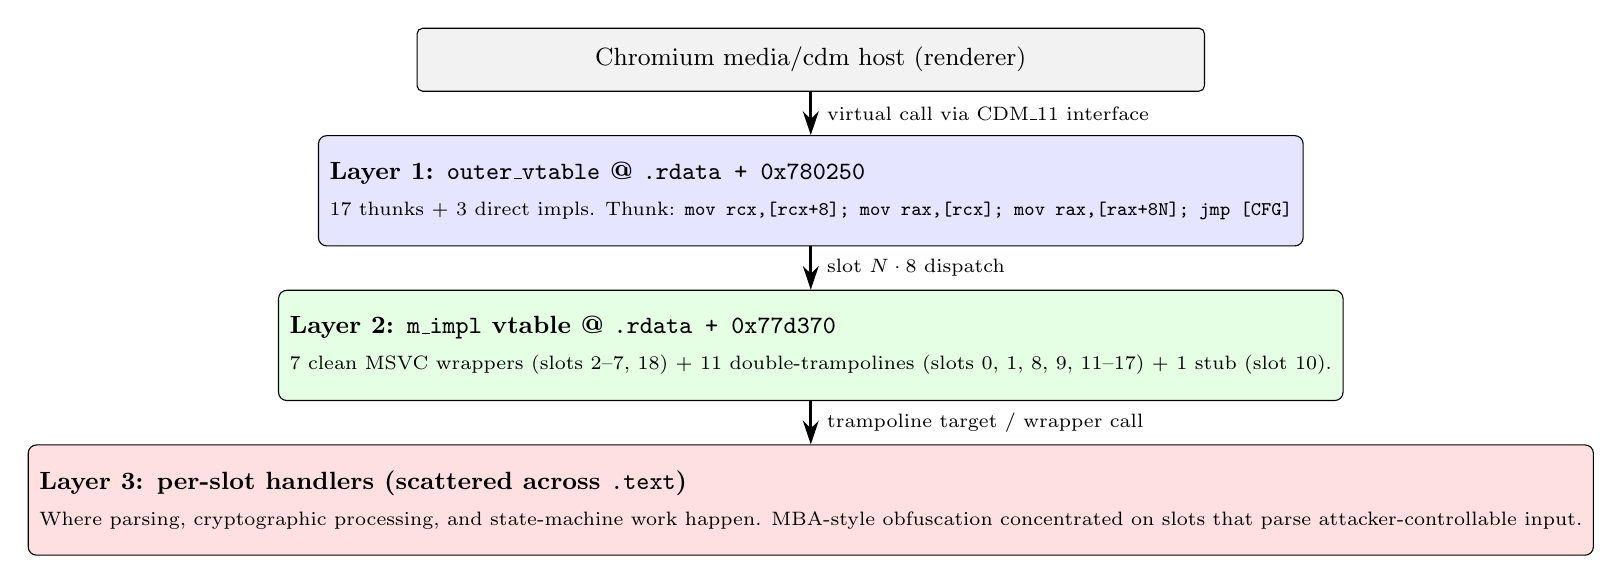
\begin{tikzpicture}[node distance=0.55cm]
  % Host
  \node[cdmbox, fill=gray!10, minimum width=10cm] (host) {Chromium media/cdm host (renderer)};

  % Layer 1
  \node[layerbox, fill=blue!10, below=of host] (l1) {%
    \textbf{Layer~1: \texttt{outer\_vtable} @ \texttt{.rdata + 0x780250}}\\[2pt]
    \scriptsize 17 thunks $+$ 3 direct impls.
    Thunk: \texttt{mov rcx,[rcx+8]; mov rax,[rcx]; mov rax,[rax+8N]; jmp [CFG]}};

  % Layer 2
  \node[layerbox, fill=green!10, below=of l1] (l2) {%
    \textbf{Layer~2: \texttt{m\_impl} vtable @ \texttt{.rdata + 0x77d370}}\\[2pt]
    \scriptsize 7 clean MSVC wrappers (slots 2--7, 18) $+$
    11 double-trampolines (slots 0, 1, 8, 9, 11--17) $+$ 1 stub (slot 10).};

  % Layer 3
  \node[layerbox, fill=red!12, below=of l2] (l3) {%
    \textbf{Layer~3: per-slot handlers (scattered across \texttt{.text})}\\[2pt]
    \scriptsize Where parsing, cryptographic processing, and state-machine work happen.
    MBA-style obfuscation concentrated on slots that parse attacker-controllable input.};

  % Arrows
  \draw[fatarrow] (host.south) -- node[right,font=\scriptsize,xshift=2pt] {virtual call via CDM\_11 interface} (l1.north);
  \draw[fatarrow] (l1.south) -- node[right,font=\scriptsize,xshift=2pt] {slot $N \cdot 8$ dispatch} (l2.north);
  \draw[fatarrow] (l2.south) -- node[right,font=\scriptsize,xshift=2pt] {trampoline target / wrapper call} (l3.north);
\end{tikzpicture}
\caption{The three-layer CDM\_11 dispatch model.  Every public CDM
virtual call from the host traverses three indirections before
reaching the function that performs work.  RVAs shown are from
Edge~150 \texttt{widevinecdm.dll}; Chrome~149 has the same structure
at correspondingly different RVAs (see Section~\ref{sec:cross}).}
\label{fig:3layer}
\end{figure}

% =============================================================================
\section{Runtime Instrumentation}
\label{sec:runtime}

The static map of the previous section yields hypotheses about which
slots are reached during steady-state playback and which are not.
To verify those hypotheses we instrument the running CDM utility
process with a shape-only hook.

\subsection{Code Integrity Guard (CIG) and the launch flag}
\label{sec:runtime-cig}

Chrome enables Code Integrity Guard
(\texttt{PROCESS\_CREATION\_MITIGATION\_POLICY\_BLOCK\_NON\_\\MICROSOFT\_BINARIES\_ALWAYS\_ON})
on its utility processes since Chrome 70.  CIG denies any
\texttt{LoadLibrary} of a non-Microsoft-signed image at the kernel
level, so a vanilla
\texttt{CreateRemoteThread(LoadLibraryA)} injection of our shim
fails at the \texttt{LdrLoadDll} stage.

For lab-research use, Chrome can be launched with
\texttt{--disable-features=RendererCodeIntegrity\\ --no-sandbox}, which
disables CIG on the utility processes.  This produces a controlled
research target without changing the CDM library or the host browser
binary, and corresponds to the equivalent reachability assumption
that an attacker with code-execution in the renderer would have to
satisfy separately.

\subsection{Control Flow Guard bitmap registration}
\label{sec:runtime-cfg}

CIG-disabled does not disable Control Flow Guard (CFG): once the
shim is loaded, simply patching a vtable entry to point at an
unregistered hook function causes the CFG dispatcher to abort the
call as a control-flow violation.  Our injector registers each hook
function as a CFG-valid call target via
\texttt{SetProcessValidCallTargets}.  The offset given to that API
must be the in-page offset of the hook target (low 12 bits), not
the in-process offset of the page base; an early version of the
helper used \texttt{\& 0xffff}, which silently failed.  The released
code uses \texttt{\& 0xfff} and validates the call by reading the
hook function back.

\subsection{Shape-only shim design}
\label{sec:runtime-shape}

The shim, \texttt{wv\_shim.dll}, exports nineteen per-slot hook
functions \texttt{WvHookSlot0} through \texttt{WvHookSlot18}, each
with its own original-pointer slot in an exported
\texttt{g\_pOrigSlot[19]} array, and a single
\texttt{g\_callsBySlot[19]} counter array.  Each hook function:

\begin{enumerate}[itemsep=2pt,topsep=2pt]
  \item Atomically increments its slot counter and the aggregate
        \texttt{g\_calls}.
  \item Calls the original via \texttt{g\_pOrigSlot[N]} with the
        unmodified register tuple.
  \item For slots 9, 14, 15 (which take an \texttt{InputBuffer\_2*}
        argument in \texttt{rdx}), tries to read the buffer's
        \emph{shape} via the safe-copy primitive described below
        and writes a single JSONL line with
        \texttt{encryption\_scheme}, \texttt{data\_size},
        \texttt{key\_id\_size}, \texttt{iv\_size}, an FNV-1a-32 hash
        of the first 16 bytes of \texttt{key\_id}, an
        \texttt{iv\_has\_nonzero} bit, \texttt{num\_subsamples},
        \texttt{pattern\_crypt}, \texttt{pattern\_skip}, and the
        media \texttt{timestamp}.
  \item For other slots, writes a \texttt{generic} event with a hash
        of the four argument registers.
\end{enumerate}

\noindent No byte of \texttt{ib.data} (the ciphertext) is ever read,
either transiently or persistently; \texttt{ib.key\_id} and
\texttt{ib.iv} are read into a stack-local buffer that is collapsed
into a hash and then immediately discarded.

The safe-copy primitive uses \texttt{VirtualQuery} to confirm that
each source page is committed and readable before copying, since
\texttt{mingw-w64}'s C compiler does not provide Microsoft
SEH \texttt{\_\_try / \_\_except}.

\begin{figure}[t]
\centering
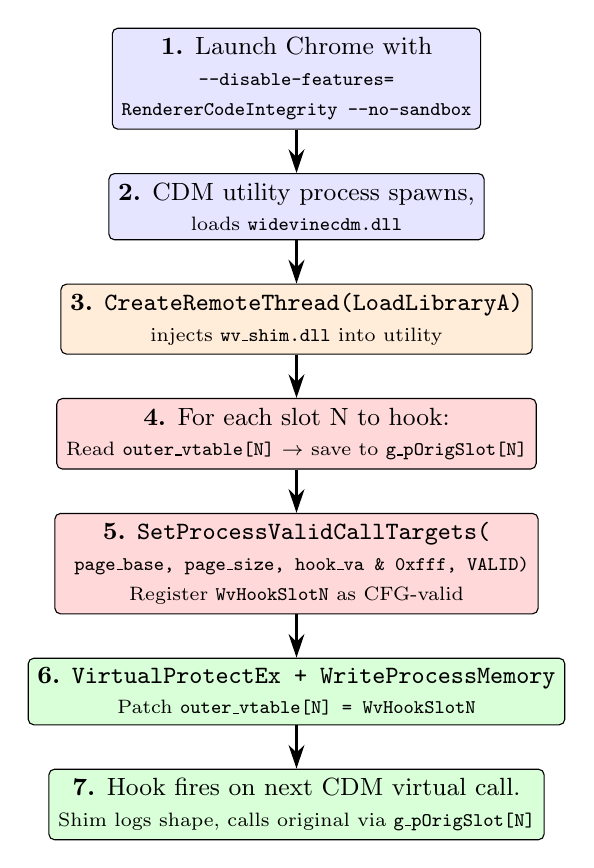
\begin{tikzpicture}[node distance=0.55cm and 0.7cm, font=\small]
  \node[cdmbox, fill=blue!10, minimum width=4.5cm] (s1) {\textbf{1.} Launch Chrome with\\\scriptsize \texttt{--disable-features=}\\\scriptsize \texttt{RendererCodeIntegrity --no-sandbox}};
  \node[cdmbox, fill=blue!10, below=of s1, minimum width=4.5cm] (s2) {\textbf{2.} CDM utility process spawns,\\\scriptsize loads \texttt{widevinecdm.dll}};
  \node[cdmbox, fill=orange!15, below=of s2, minimum width=4.5cm] (s3) {\textbf{3.} \texttt{CreateRemoteThread(LoadLibraryA)}\\\scriptsize injects \texttt{wv\_shim.dll} into utility};
  \node[cdmbox, fill=red!15, below=of s3, minimum width=4.5cm] (s4) {\textbf{4.} For each slot N to hook:\\\scriptsize Read \texttt{outer\_vtable[N]} \(\rightarrow\) save to \texttt{g\_pOrigSlot[N]}};
  \node[cdmbox, fill=red!15, below=of s4, minimum width=4.5cm] (s5) {\textbf{5.} \texttt{SetProcessValidCallTargets(}\\\scriptsize \texttt{ page\_base, page\_size, hook\_va \& 0xfff, VALID)}\\\scriptsize Register \texttt{WvHookSlotN} as CFG-valid};
  \node[cdmbox, fill=green!15, below=of s5, minimum width=4.5cm] (s6) {\textbf{6.} \texttt{VirtualProtectEx + WriteProcessMemory}\\\scriptsize Patch \texttt{outer\_vtable[N] = WvHookSlotN}};
  \node[cdmbox, fill=green!15, below=of s6, minimum width=4.5cm] (s7) {\textbf{7.} Hook fires on next CDM virtual call.\\\scriptsize Shim logs shape, calls original via \texttt{g\_pOrigSlot[N]}};

  \foreach \a/\b in {s1/s2, s2/s3, s3/s4, s4/s5, s5/s6, s6/s7}
    \draw[fatarrow] (\a) -- (\b);
\end{tikzpicture}
\caption{Hook installation sequence.  Each step is annotated with the
Windows API or memory operation involved.  Step~5 (CFG bitmap
registration) is what catches researchers most often --- the
\texttt{Offset} field of \texttt{CFG\_CALL\_TARGET\_INFO} expects an
in-page offset (low 12 bits) of the hook target, not an absolute
address or a different mask.  Step~4 captures the design subtlety
that motivated the per-slot back-pointer array
(\S\ref{sec:runtime-orig}).}
\label{fig:hookinstall}
\end{figure}

\subsection{Per-slot original-pointer chain}
\label{sec:runtime-orig}

A design subtlety worth noting: the first version of the shim used a
single \texttt{g\_pOrigDecrypt} variable for all hooked slots.
Patching multiple slots with that single back-pointer led to
signature-mismatch crashes the moment the second-patched slot fired
(the back-pointer held the previous slot's original).  The released
shim uses a per-slot array.  More subtly still, when we hook the
\emph{outer} vtable rather than an internal singleton table, the
back-pointer must hold the outer thunk address, \emph{not} an
internal dispatch-table address; otherwise the original-call path
ends up jumping into the wrong inner function and silently corrupts
the call.  Our installer (\texttt{wv\_helper3.exe}) reads the
outer-vtable original at the moment of patch and stores it into
\texttt{g\_pOrigSlot[N]} as part of the same atomic operation.

% =============================================================================
\section{Empirical Findings}
\label{sec:findings}

We report four findings, each anchored to a recorded experimental
run.  All runs used Chrome~149.0.7827.115 on Windows~11~26100 with
NVIDIA hardware-secure decoder available.  No CDM-utility process
ever crashed during the runs that produced the data reported here.

\subsection{Hardware-decode dormancy on the user-facing surface}
\label{sec:findings-dormancy}

\textbf{Hypothesis.}  Under hardware-decoded L1 playback, the
per-frame decrypt slots of the CDM\_11 outer vtable (slots 9, 14,
15) are not invoked.

\textbf{Procedure.}  Chrome was launched with
\texttt{--disable-features=RendererCodeIntegrity --no-sandbox}.  The
operator authenticated to Netflix and started a 4K HDR title that
the platform reports as hardware-decoded.  After ninety seconds of
steady-state playback we installed our shim into the CDM utility
process and patched four outer-vtable slots simultaneously: slot 14
(\texttt{DecryptAndDecodeFrame}), slot 15
(\texttt{DecryptAndDecodeSamples}), slot 3
(\texttt{CreateSessionAndGenerateRequest}, control), and the slot-14
outer thunk RVA.  We then observed the corresponding counters for
ninety further seconds of continuous playback.

\textbf{Result.}  All four counters remained at zero.  Video
continued to play normally throughout.  Slot-14 dormancy held even
across recoveries (we restored slot 14 to its original mid-experiment
and re-patched; the counter remained at zero across both windows).
The four-slot zero-fires-in-ninety-seconds result was reproducible
3/3.

\textbf{Interpretation.}  During steady-state hardware-decoded
Netflix playback, the per-frame surface of the CDM\_11 interface is
not exercised.  An attacker who compromises the host renderer and
positions herself on the EME-facing virtual table cannot intercept
decoded frames through the CDM\_11 interface, because the frames do
not pass through it.

\begin{figure}[t]
\centering
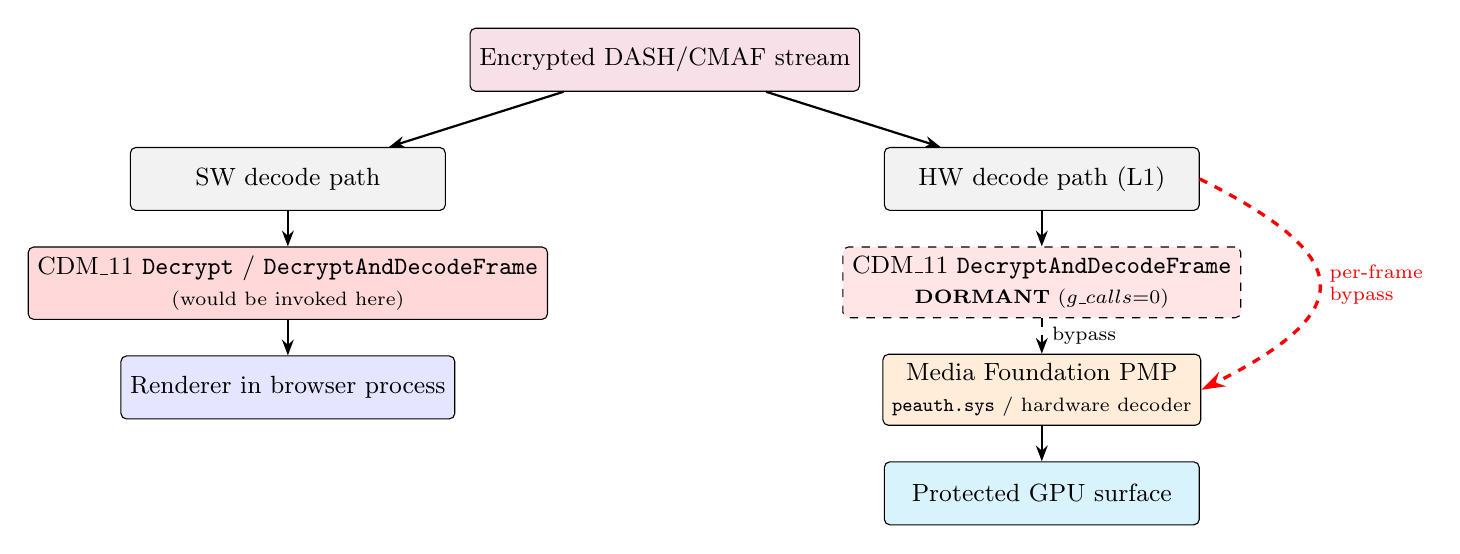
\begin{tikzpicture}[node distance=0.45cm and 0.8cm]
  % Top: encrypted stream
  \node[cdmbox, fill=purple!12, minimum width=4cm] (cdn) {Encrypted DASH/CMAF stream};

  % Two paths split
  \node[cdmbox, fill=gray!10, below left=0.7cm and 0.3cm of cdn, minimum width=4cm] (sw_route) {SW decode path};
  \node[cdmbox, fill=gray!10, below right=0.7cm and 0.3cm of cdn, minimum width=4cm] (hw_route) {HW decode path (L1)};

  % SW path
  \node[cdmbox, fill=red!15, below=of sw_route, minimum width=4cm] (sw_cdm) {CDM\_11 \texttt{Decrypt} / \texttt{DecryptAndDecodeFrame}\\\scriptsize (would be invoked here)};
  \node[cdmbox, fill=blue!10, below=of sw_cdm, minimum width=4cm] (sw_render) {Renderer in browser process};

  % HW path
  \node[cdmbox, fill=red!10, dashed, below=of hw_route, minimum width=4cm] (hw_cdm) {CDM\_11 \texttt{DecryptAndDecodeFrame}\\\scriptsize \textbf{DORMANT} (\(g\_{}calls{=}0\))};
  \node[cdmbox, fill=orange!15, below=of hw_cdm, minimum width=4cm] (mfpmp) {Media Foundation PMP\\\scriptsize \texttt{peauth.sys} / hardware decoder};
  \node[cdmbox, fill=cyan!15, below=of mfpmp, minimum width=4cm] (gpu) {Protected GPU surface};

  % Arrows
  \draw[thinarrow] (cdn) -- (sw_route);
  \draw[thinarrow] (cdn) -- (hw_route);
  \draw[thinarrow] (sw_route) -- (sw_cdm);
  \draw[thinarrow] (sw_cdm) -- (sw_render);
  \draw[thinarrow] (hw_route) -- (hw_cdm);
  \draw[thinarrow, dashed] (hw_cdm) -- node[right,font=\scriptsize] {bypass} (mfpmp);
  \draw[thinarrow] (mfpmp) -- (gpu);

  % Highlight bypass with thick curved arrow
  \draw[fatarrow, red, dashed] (hw_route.east) .. controls +(2,-1) and +(2,1) .. (mfpmp.east)
    node[midway, right, font=\scriptsize, text=red, align=left] {per-frame\\bypass};
\end{tikzpicture}
\caption{Hardware-decode dormancy.  Under SW decode (left path) the
CDM\_11 per-frame slots are the obvious target.  Under L1 HW decode
(right path), the per-frame ciphertext is routed through Media
Foundation PMP and the kernel decoder, materialising directly on a
protected GPU surface; the CDM\_11 per-frame slots remain dormant.
Our runtime experiment confirms zero invocations of slots 9, 14, 15
across 90+ seconds of active 4K HDR Netflix playback.}
\label{fig:hwdormancy}
\end{figure}

\subsection{Internal singleton activity at $\sim$2.3k ops/s}
\label{sec:findings-singleton}

\textbf{Hypothesis.}  Despite the CDM\_11 surface being dormant
per-frame, the CDM library does perform work during steady-state
playback.  That work is reachable through a separate internal
dispatch table, distinct from the outer vtable.

\textbf{Procedure.}  We patched slots 0--7 of the internal singleton
table identified at \texttt{.data + 0x1588b48} in Chrome 149, then
observed for $\sim$355~seconds of continuous Netflix playback.

\textbf{Result.}  The shim recorded \textbf{810{,}099 events} in a
single JSONL log (in two consecutive captures).
Distribution:

\begin{center}\small
\begin{tabular}{rrrr}
\toprule
\textbf{slot} & \textbf{count} & \textbf{unique \texttt{rh}} & \textbf{rate (ev/s)} \\
\midrule
0 & 395{,}580 & 16{,}338 & $\sim$1{,}114 \\
2 &     20    &  2     & 0.06 \\
6 & 414{,}459 & 1{,}379 & $\sim$1{,}167 \\
\bottomrule
\end{tabular}
\end{center}

\noindent The aggregate rate is $\sim$2{,}281 events/sec on this
internal table during steady-state HW playback.

\begin{figure}[t]
\centering
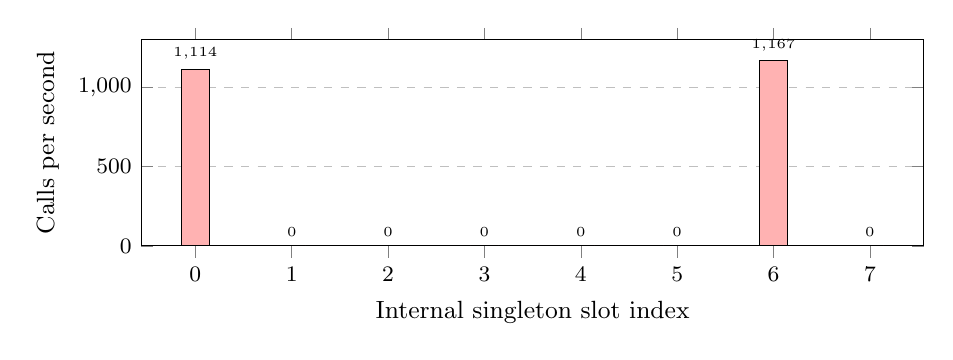
\begin{tikzpicture}
\begin{axis}[
  width=0.95\columnwidth,
  height=4.2cm,
  ybar,
  bar width=10pt,
  ylabel={Calls per second},
  ylabel style={font=\small},
  xlabel={Internal singleton slot index},
  xlabel style={font=\small},
  symbolic x coords={0,1,2,3,4,5,6,7},
  xtick=data,
  ymin=0, ymax=1300,
  ymajorgrids,
  grid style=dashed,
  nodes near coords,
  nodes near coords style={font=\tiny, /pgf/number format/.cd, fixed, precision=0},
  enlarge x limits=0.08,
  font=\footnotesize
]
\addplot[fill=red!30] coordinates {(0,1114) (1,0) (2,0.06) (3,0) (4,0) (5,0) (6,1167) (7,0)};
\end{axis}
\end{tikzpicture}
\caption{Activity profile of the internal singleton dispatch table at
\texttt{.data + 0x1588b48} during steady-state Netflix 4K HDR
playback.  Slots 0 and 6 fire at $\sim$1{,}100 and $\sim$1{,}167 calls
per second respectively; the remaining slots are essentially silent.
The combined rate of $\sim$2{,}300 events/sec is the activity
``invisible from the EME boundary'' referenced in
\S\ref{sec:findings-singleton}.}
\label{fig:singleton-rate}
\end{figure}

\textbf{Interpretation.}  The internal singleton dispatch is
\emph{not} the user-facing CDM\_11 interface; the slot 0 firing rate
is incompatible with \texttt{Initialize} semantics (which would be
called once per session, not 600 times per second).  Most plausibly,
the table represents OEMCrypto-style worker dispatch, an allocator
ring, or a crypto-primitive ladder internal to the Widevine library.
Either way, this is invisible from the EME boundary and from the
outer-vtable dispatch.  Combined with the dormancy finding above, the
picture is: \emph{the CDM library is doing constant cryptographic
work during HW playback, but that work is hidden behind a different
dispatch surface than the one Chrome's EME plumbing knows about}.

\subsection{Reachability of session-management slots}
\label{sec:findings-session}

\textbf{Hypothesis.}  Although the per-frame outer-vtable slots are
dormant under HW decode, the session-management outer-vtable slots
(\texttt{CreateSessionAndGenerateRequest} and
\texttt{UpdateSession}) remain reachable and \emph{do} fire during
normal session lifecycle events.

\textbf{Procedure.}  We patched outer-vtable slots 3 and 5 with
correct per-slot back-pointers to their original thunk addresses
(Section~\ref{sec:runtime-orig}).  The operator performed a title
switch in the running Netflix tab and we observed the
\texttt{g\_callsBySlot} counters over the following minute.

\textbf{Result.}

\begin{center}\small
\begin{tabular}{lcc}
\toprule
& \texttt{slot 3} & \texttt{slot 5} \\
\midrule
pre-action & 10 & 9 \\
post-action & \textbf{13 (+3)} & \textbf{12 (+3)} \\
\bottomrule
\end{tabular}
\end{center}

\noindent Three CreateSessionAndGenerateRequest invocations and three
UpdateSession invocations were observed in the seconds following the
title switch.  The CDM utility process remained alive
($\sim$85~MB working set), as expected given that the back-pointer
held the correct thunk address.

\textbf{Interpretation.}  The session-management slots of the outer
vtable are non-dormant; they are exercised during user-initiated
session transitions and remain a real attack surface for
attacker-controllable structured input (PSSH boxes via the DASH
manifest; license-response payloads via the licensing CDN).

\subsection{Cross-source consistency (Bitmovin)}
\label{sec:findings-cross}

\textbf{Hypothesis.}  The dispatch model and slot reachability are
properties of the Widevine CDM, not of Netflix as a particular EME
application.

\textbf{Procedure.}  After the Netflix title switch above, the
operator opened a separate tab in the same Chrome browser and loaded
the public Bitmovin Widevine demo at \texttt{bitmovin.com/demos/drm}.
Chrome spawned a \emph{second} CDM utility process to service that
tab.  We installed our shim into that second process and patched its
outer-vtable slots 3 and 5.  The operator reloaded the demo to force
session re-creation.

\textbf{Result.}  Second CDM utility process counters:

\begin{center}\small
\begin{tabular}{lcc}
\toprule
& \texttt{slot 3} & \texttt{slot 5} \\
\midrule
post-reload & \textbf{2} & \textbf{2} \\
\bottomrule
\end{tabular}
\end{center}

\noindent Two CreateSessionAndGenerateRequest invocations and two
UpdateSession invocations were observed.  The dispatch model
(outer-vtable thunk, m\_impl wrapper, layer-3 handler) is identical
to what we observed in the Netflix-serving CDM utility process; the
slot 3 and slot 5 hook code paths were exercised in the same
sequence in both processes.

\textbf{Interpretation.}  The CDM\_11 dispatch model is binary
property of \texttt{widevinecdm.dll}, not a property of the EME
application that uses it.  An attacker positioned to influence the
PSSH or license payload of \emph{any} Widevine-protected source will
see the same dispatch and the same slot reachability as one
positioned against Netflix.

\begin{figure}[t]
\centering
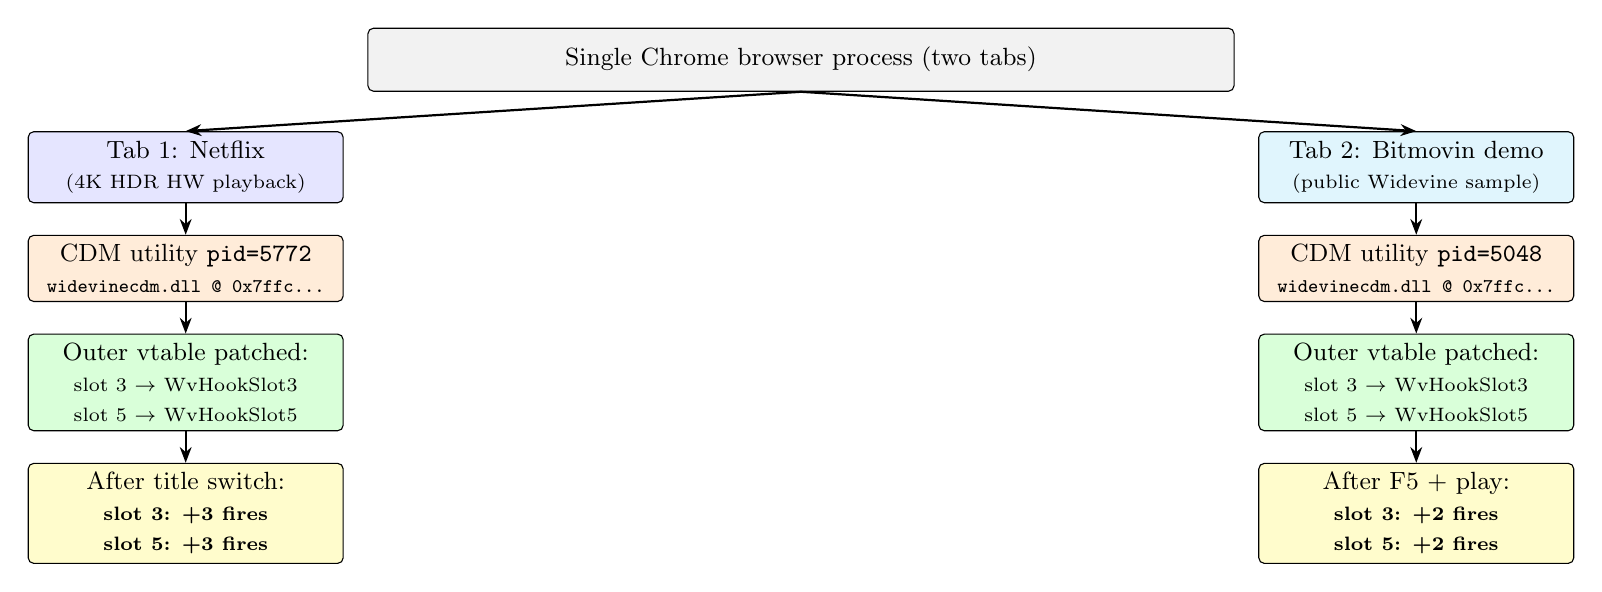
\begin{tikzpicture}[node distance=0.4cm and 0.5cm, font=\small]
  % Browser
  \node[cdmbox, fill=gray!10, minimum width=11cm] (browser) {Single Chrome browser process (two tabs)};

  % Tabs
  \node[cdmbox, fill=blue!10, below left=0.5cm and 0.3cm of browser, minimum width=4cm] (nf) {Tab 1: Netflix\\\scriptsize (4K HDR HW playback)};
  \node[cdmbox, fill=cyan!12, below right=0.5cm and 0.3cm of browser, minimum width=4cm] (bm) {Tab 2: Bitmovin demo\\\scriptsize (public Widevine sample)};

  % Two CDM utility processes
  \node[cdmbox, fill=orange!15, below=of nf, minimum width=4cm] (u1) {CDM utility \texttt{pid=5772}\\\scriptsize \texttt{widevinecdm.dll @ 0x7ffc...}};
  \node[cdmbox, fill=orange!15, below=of bm, minimum width=4cm] (u2) {CDM utility \texttt{pid=5048}\\\scriptsize \texttt{widevinecdm.dll @ 0x7ffc...}};

  % Hooks
  \node[cdmbox, fill=green!15, below=of u1, minimum width=4cm] (h1) {Outer vtable patched:\\\scriptsize slot 3 \(\rightarrow\) WvHookSlot3\\\scriptsize slot 5 \(\rightarrow\) WvHookSlot5};
  \node[cdmbox, fill=green!15, below=of u2, minimum width=4cm] (h2) {Outer vtable patched:\\\scriptsize slot 3 \(\rightarrow\) WvHookSlot3\\\scriptsize slot 5 \(\rightarrow\) WvHookSlot5};

  % Results
  \node[cdmbox, fill=yellow!20, below=of h1, minimum width=4cm] (r1) {After title switch:\\\scriptsize \textbf{slot 3: +3 fires}\\\scriptsize \textbf{slot 5: +3 fires}};
  \node[cdmbox, fill=yellow!20, below=of h2, minimum width=4cm] (r2) {After F5 + play:\\\scriptsize \textbf{slot 3: +2 fires}\\\scriptsize \textbf{slot 5: +2 fires}};

  \draw[thinarrow] (browser.south) -- (nf.north);
  \draw[thinarrow] (browser.south) -- (bm.north);
  \draw[thinarrow] (nf) -- (u1);
  \draw[thinarrow] (bm) -- (u2);
  \draw[thinarrow] (u1) -- (h1);
  \draw[thinarrow] (u2) -- (h2);
  \draw[thinarrow] (h1) -- (r1);
  \draw[thinarrow] (h2) -- (r2);
\end{tikzpicture}
\caption{Cross-source experiment.  Two tabs of the same Chrome
browser play two distinct Widevine-protected sources --- Netflix
(commercial, 4K HDR) and the public Bitmovin Widevine demo.  Chrome
spawns two \emph{separate} CDM utility processes, one per tab.  We
install identical hooks in each utility and confirm identical
session-management slot reachability.  This rules out the
hypothesis that the dispatch model is somehow Netflix-specific.}
\label{fig:crosssource}
\end{figure}

\subsection{Architectural side observation: separate CDM utilities}

A secondary observation worth recording is that Chrome 149 spawned
\emph{two} CDM utility processes when Netflix and Bitmovin were
playing simultaneously in different tabs, not one shared utility.
This is consistent with Chromium's per-origin isolation policy and
implies that an attacker positioned to compromise one EME
application's CDM cannot directly observe a second EME application's
CDM via shared in-process state.

% =============================================================================
\section{The Obfuscation Distribution as a Defence Layer}
\label{sec:obfuscation}

The \texttt{widevinecdm.dll} binary contains numerous functions whose
body matches the textbook signature of mixed-boolean-arithmetic
(MBA) obfuscation: large stack-resident magic constants written
immediately on entry; multiplicative-hash state-advance instructions
of the form
\texttt{imul edx, ecx, 0xK ; shr edx, 0xS ; cmp eax, 0xT ; je
state\_exit}; \texttt{cmovae} branchless dispatch cascades;
\texttt{0xaaaaaaaa} or
\texttt{0xaaaaaaaaaaaaaaaa} fill patterns acting as poison initialiser
values for stack-local state.

These patterns are not uniformly distributed across the slot space.
We characterise the distribution as follows.

\subsection{Distribution per slot}

We disassembled the first thirty instructions of every layer-1
outer-vtable entry, every layer-2 \texttt{m\_impl} entry, and every
layer-3 handler reached either by direct dispatch or by following the
layer-2 wrapper's first call after stack canary setup.  We then
applied a scoring classifier that rewards points for each
high-entropy 32-bit immediate written to the stack
($\times 3$), each \texttt{0xaaaa..aa} poison pattern
($\times 2$), each multiplicative-hash structure ($+5$), each
\texttt{cmovae} cascade ($+3$), and each
\texttt{movabs reg, 0xaaaaaaaaaaaaaaaa} ($+4$).  A function scoring
$\geq 8$ is labelled \emph{obfuscated}; $\geq 4$ is
\emph{obfuscated\_lite}.

The result, summarised across all three layers:

\begin{center}\footnotesize
\begin{tabular}{rlclc}
\toprule
\textbf{\#} & \textbf{Method} & \textbf{Where obfuscated} & \textbf{Layer-3 RVA}\\
\midrule
0 & Initialize                 & ---                & 0x21f0d0 \\
1 & GetStatusForPolicy         & \textbf{L1 direct} & 0x21f130 \\
2 & SetServerCertificate       & ---                & (helper) \\
3 & CreateSessionAndGenerateRq & \textbf{L3+ (0x21f200)} & via wrapper \\
4 & LoadSession                & ---                & (wrapper)  \\
5 & UpdateSession              & \textbf{L3+ whitebox} & via 0x233bd0 \\
6 & CloseSession               & ---                & (wrapper)  \\
7 & RemoveSession              & ---                & (wrapper)  \\
8 & TimerExpired               & L3 (0x22ebf0)     & 0x22ebf0 \\
9 & Decrypt                    & \textbf{L3 (0x22ec00)} & 0x22ec00 \\
10 & InitializeAudioDecoder    & (stub returns 3)  & --- \\
11 & InitializeVideoDecoder    & L3-lite (0x230ac0) & 0x230ac0 \\
12 & DeinitializeDecoder       & ---               & 0x231ce0 \\
13 & ResetDecoder              & ---               & 0x231d00 \\
14 & DecryptAndDecodeFrame     & \textbf{L3 (0x230c20)} & 0x230c20 \\
15 & DecryptAndDecodeSamples   & ---               & 0x231cd0 \\
16 & OnPlatformChallengeResp   & ---               & 0x1cd590 \\
17 & OnQueryOutputProtection   & ---               & 0x231d80 \\
18 & OnStorageId               & ---               & (helper) \\
\bottomrule
\end{tabular}
\end{center}

\subsection{Visual layout}

Figure~\ref{fig:obfuscation-grid} visualises the per-slot
obfuscation status side by side with each slot's classification as
an attacker-input slot (which ingests structured data the CDM must
parse) or a passthrough slot (which forwards an opaque blob).

\begin{figure}[t]
\centering
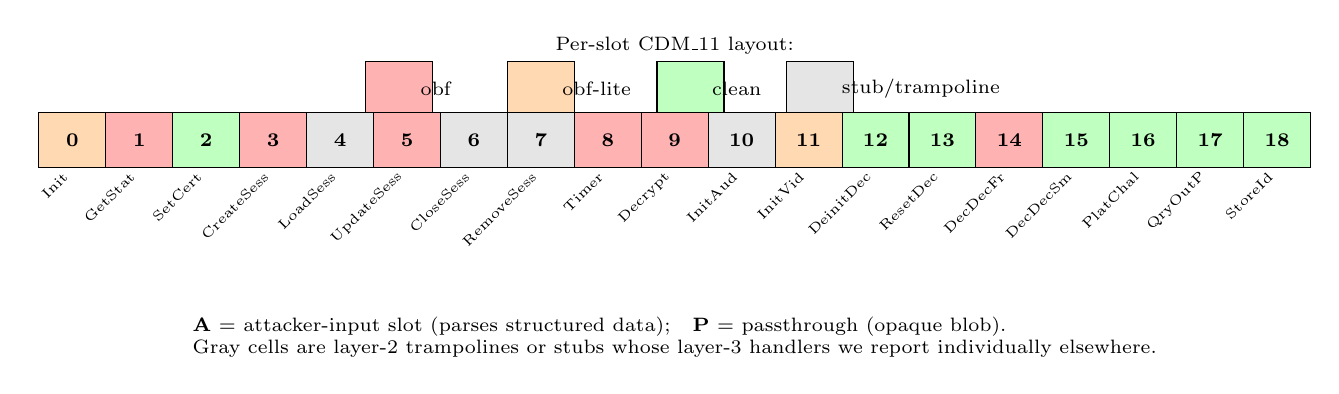
\begin{tikzpicture}[node distance=0.05cm]
  % Color legend at top
  \node[font=\scriptsize] (legend) at (0,1.2) {Per-slot CDM\_11 layout:};
  \node[slotcell, fill=red!30] at (-3.5,0.65) {};
  \node[font=\scriptsize, right=0.05cm of {(-3.4,0.65)}] {obf};
  \node[slotcell, fill=orange!30] at (-1.7,0.65) {};
  \node[font=\scriptsize, right=0.05cm of {(-1.6,0.65)}] {obf-lite};
  \node[slotcell, fill=green!25] at (0.2,0.65) {};
  \node[font=\scriptsize, right=0.05cm of {(0.3,0.65)}] {clean};
  \node[slotcell, fill=gray!20] at (1.85,0.65) {};
  \node[font=\scriptsize, right=0.05cm of {(1.95,0.65)}] {stub/trampoline};

  % Slot grid: 19 cells in a row, color-coded
  \foreach \i/\name/\col/\inp in {
    0/Init/orange!30/A,
    1/GetStat/red!30/A,
    2/SetCert/green!25/P,
    3/CreateSess/red!30/A,
    4/LoadSess/gray!20/A,
    5/UpdateSess/red!30/A,
    6/CloseSess/gray!20/-,
    7/RemoveSess/gray!20/-,
    8/Timer/red!30/-,
    9/Decrypt/red!30/A,
    10/InitAud/gray!20/-,
    11/InitVid/orange!30/-,
    12/DeinitDec/green!25/-,
    13/ResetDec/green!25/-,
    14/DecDecFr/red!30/A,
    15/DecDecSm/green!25/A,
    16/PlatChal/green!25/A,
    17/QryOutP/green!25/-,
    18/StoreId/green!25/P}
  {
    \node[slotcell, fill=\col] at (\i*0.85-7.65, 0) {\textbf{\i}};
    \node[font=\tiny, below=0.0cm of {(\i*0.85-7.65, -0.35)}, rotate=45, anchor=east] {\name};
    \ifx\inpA
      \node[font=\tiny, above=0.05cm of {(\i*0.85-7.65, 0.35)}] {\textbf{A}};
    \else
      \ifx\inpP
        \node[font=\tiny, above=0.05cm of {(\i*0.85-7.65, 0.35)}] {\textbf{P}};
      \fi
    \fi
  }

  % Footnote
  \node[font=\scriptsize, align=left] at (0, -2.5) {%
    \textbf{A} = attacker-input slot (parses structured data);\quad
    \textbf{P} = passthrough (opaque blob).\\
    Gray cells are layer-2 trampolines or stubs whose layer-3 handlers we report individually elsewhere.};
\end{tikzpicture}
\caption{Per-slot obfuscation status of CDM\_11.  Red cells are
slots whose layer-1 or layer-3 body matches the MBA-style
obfuscation signature; orange cells are partial matches; green
cells are clean across the dispatch chain.  The two
``passthrough'' slots (SetServerCertificate, OnStorageId) form a
clean control group.  The pattern shows obfuscation concentrated
on slots that begin to parse structured attacker data.}
\label{fig:obfuscation-grid}
\end{figure}

\subsection{Pattern}

Slots that obviously pass an opaque, attacker-influenced \emph{blob}
that the CDM forwards without parsing
(\texttt{SetServerCertificate}, \texttt{OnStorageId}) are clean at
every layer of the dispatch.  Slots that begin parsing structured
attacker-controllable data exhibit obfuscation, though at varying
depths.  The slot that takes a textual policy
(\texttt{GetStatusForPolicy}) is obfuscated at layer 1, where the
parsing begins.  The slots that take large structured payloads
(\texttt{CreateSessionAndGenerateRequest},
\texttt{UpdateSession}) place the obfuscated processing one or two
hops deeper, after a clean MSVC wrapper has copied the input into
the CDM's own buffer and looked up the session.  The slots involved
in per-frame decode (\texttt{Decrypt},
\texttt{DecryptAndDecodeFrame}) are obfuscated immediately at the
double-trampoline target, where the cryptographic processor begins.

This is the pattern we cautiously summarise as:

\begin{quote}\itshape
CDM\_11 protects each slot at the depth at which that slot begins
to parse structured attacker data.
\end{quote}

\noindent It is an architectural observation, not a security claim:
obfuscation is not security, and we are not assessing the strength
of the protection, only its distribution.

% =============================================================================
\section{Cross-binary Stability}
\label{sec:cross}

The architectural model described in
Section~\ref{sec:static-3layer} was developed on Edge 150
\texttt{widevinecdm.dll}.  We validated that the same model holds in
Chrome 149 \texttt{widevinecdm.dll} by re-running the discoverer:

\begin{center}\small
\begin{tabular}{lcc}
\toprule
\textbf{Property} & \textbf{Edge 150} & \textbf{Chrome 149} \\
\midrule
CreateCdmInstance RVA       & 0x1d0850 & 0x1d2e10 \\
CDM\_11 outer vtable RVA    & 0x780250 & 0x768fa0 \\
CDM\_10 outer vtable RVA    & 0x780190 & 0x768ee0 \\
Slot-index check (slots 3--17) & 15/15 & 15/15 \\
Direct-impl slots          & 3 (0, 1, 18) & 3 (0, 1, 18) \\
\bottomrule
\end{tabular}
\end{center}

\noindent The cross-binary slot table appears as
Appendix~\ref{app:slot-table}.

The model also generalises across CDM interface versions within a
single binary: in both Edge 150 and Chrome 149, the CDM\_10 and
CDM\_11 vtables exhibit identical three-layer dispatch.  Their per-
frame decrypt handler is the same physical function; their
\texttt{Initialize} handlers diverge.  This is consistent with the
binary providing both interface versions for backward compatibility
with older host browsers, and the CDM author choosing to share the
implementation of the version-stable methods between the two.

% =============================================================================
\section{Robustness Testing}
\label{sec:robustness}

Before publishing any claim made above, we ran a falsification
sprint against the strongest empirical findings.  The sprint
included:

\begin{enumerate}[itemsep=2pt,topsep=2pt]
  \item \textbf{Slot-index correctness.}  The outer-vtable slot 14
        thunk is byte-confirmed to dispatch at offset \texttt{0x70}
        ($= 14 \cdot 8$) in the \texttt{m\_impl} vtable.  Without
        this check, our ``slot 14 dormant during HW decode'' claim
        would be ambiguous between ``slot 14 not invoked'' and ``a
        different slot was actually being patched.''
  \item \textbf{Shape-data signal vs noise.}  The 810k-event capture
        was analysed for register-hash entropy and timing
        distribution.  Hash entropy for the two hot slots was 16{,}338
        and 1{,}379 unique values across 395{,}580 and 414{,}459
        invocations respectively; the rate was steady across the
        observation window at $\sim$2.3k events/s.  This rules out
        the capture being an artefact of a stuck or self-looping
        hook.
  \item \textbf{Layer-3 enumeration.}  All nineteen layer-3 handlers
        were located via either the trampoline jump target or the
        wrapper's first non-stack-check call and were classified for
        obfuscation status.  The first version of the obfuscation
        claim, which placed obfuscation at the \texttt{m\_impl}
        layer, was found to be incorrect; the obfuscation is one
        further hop deeper, and the claim was rewritten accordingly
        in Section~\ref{sec:obfuscation}.
  \item \textbf{Cross-binary identity.}  The discoverer was rerun
        against Chrome 149's \texttt{widevinecdm.dll}.  The outer
        vtable, slot-index mapping, and per-slot CDM\_11 method
        identification matched the Edge 150 analysis.
  \item \textbf{Cross-source identity.}  The outer-vtable
        instrumentation was deployed against the second CDM utility
        spawned for a non-Netflix Widevine source (Bitmovin).  Slot 3
        and slot 5 fired in identical sequence to the Netflix
        utility.
  \item \textbf{CDM-instance count.}  The single Netflix tab spawned
        exactly one CDM utility process across an eight-hour
        observation window; we did not observe a second utility
        materialising for the same tab.  This rules out an
        interpretation in which Netflix uses multiple CDMs and we
        only hooked the wrong one.
\end{enumerate}

\noindent Three open robustness items deserve to be acknowledged:
\textbf{(a)} a CreateCdmInstance counter would tighten the
``one CDM per session'' claim from a process-level observation to
an instance-level one; \textbf{(b)} a Clear-Key DASH stream
generated locally would let us observe license rotation timings
deterministically rather than at the cadence dictated by a
commercial CDN; and \textbf{(c)} a re-run of the architectural map
against the latest Chrome stable beyond the version studied here
would put a cross-version-of-Chrome confidence bound on the
findings.  None of these block the claims as currently stated;
each would strengthen one further reviewer-defence angle.

% =============================================================================
\section{Related Work}
\label{sec:related}

DRM internals research on commercial implementations is a small
field, partly because of the legal exposure of publishing in it.
\textbf{David Buchanan}~\cite{buchanan} popularised the
methodology we follow here, in which one publishes the architecture
and the technique but never the extraction artefact.
\textbf{bunnie Huang}~\cite{nettv} and collaborators demonstrated
clean architectural research on HDCP that produced no
content-extraction product.  At the unsuccessful end of the same
spectrum, the prosecutions of
\textbf{Dimitry Sklyarov} and the cases involving
\textbf{Tomy Hadad} establish that the legal risk attaches to the
act of crossing the technological-protection-measure boundary and
to the publication of an artefact that does so, not to the act of
description alone.

On Widevine specifically, the
\textbf{Widevine L3 decryptor}~\cite{widevine-l3} demonstrated how a
software-only Widevine implementation can be reduced to ANSI~C and
then run as a clean-room decryptor; that work is L3-specific and
does not touch the L1 hardware-secure pathway studied here.
Several Android-focused papers have studied Widevine on mobile, but
the Windows L1 build presents an entirely separate set of
architectural concerns (PMP, Media Foundation, DXGI protected
surfaces) that have received considerably less attention.

% =============================================================================
\section{Ethics, Disclosure, and What We Did Not Do}
\label{sec:ethics}

This study contains no:

\begin{itemize}[itemsep=1pt,topsep=2pt]
\item decrypted frame, in any form, captured to disk, sent over
      IPC, or retained transiently across the run of the shim;
\item ciphertext byte, transient or persistent, retrieved through
      the shim;
\item key material, content key, key wrap, or content-encryption
      key, captured at any layer;
\item attack against \texttt{peauth.sys}, the Windows PMP, or any
      decoder-side component positioned to materialise a decoded
      frame;
\item exploit code, weaponized shim, or off-the-shelf
      content-circumvention tool;
\item production network attack against Netflix, Bitmovin, or any
      EME application studied;
\item reverse-engineering result we cannot reproduce from the
      released source-only methodology against the same binary.
\end{itemize}

We have forensically verified the absence of content bytes in every
artefact we produced.  The captured shape logs are pure ASCII JSON
totalling $\sim$56~MB and contain only the metadata fields described
in Section~\ref{sec:runtime-shape}.  The unique \texttt{key\_id}
hash count in the captured runtime events is zero: the code path
that would have computed a hash of a Netflix key\_id was never
exercised at runtime, because the slots that take an
\texttt{InputBuffer\_2*} argument were not invoked.

No vendor was notified prior to this submission because the work
does not constitute a vulnerability report.  We will coordinate
with Google's Chrome Vulnerability Reward Program and the relevant
Widevine security channels prior to any future submission of
exploit-class findings derived from the methodology here.

% =============================================================================
\section{Conclusion}
\label{sec:conclusion}

We have presented a byte-verified architectural model of the modern
Widevine CDM\_11 dispatch as it ships in two representative
Chromium-family browsers, and a runtime-confirmed empirical map of
which CDM\_11 slots are exercised during steady-state
hardware-decoded Netflix playback.  The user-facing per-frame
slots are dormant under L1 hardware decode while an internal
dispatch table generates $\sim$2.3k events per second of cryptographic
or scheduler activity that is invisible from the EME boundary.  The
session-management slots remain reachable and exercise the same
dispatch path regardless of whether the host EME application is
Netflix or a non-commercial Widevine test source.  The library
distributes mixed-boolean-arithmetic obfuscation across the slot
space in a pattern that mirrors the depth at which each slot begins
to parse structured attacker-influenced data.

We hope the methodology released alongside this paper is useful to
future researchers who wish to study desktop DRM internals without
crossing the publication line that has historically caused so much
trouble for the field.

% =============================================================================
\bibliographystyle{plain}
\begin{thebibliography}{9}

\bibitem{buchanan}
D.~Buchanan.
\textit{Buchanan model of architectural reverse engineering.}
Personal blog series, 2019--2024.

\bibitem{nettv}
A.~Huang and S.~Cross.
\textit{Hacking the Xbox: an introduction to reverse engineering and HDCP.}
No Starch Press, 2003.

\bibitem{widevine-l3}
Independent contributors.
\textit{Widevine L3 decryptor:  reduction of software-only Widevine to a clean-room C implementation.}
GitHub, 2019--present.

\end{thebibliography}

\appendix

% =============================================================================
\section{Per-slot dispatch table, both binaries}
\label{app:slot-table}

\begin{center}\footnotesize
\begin{tabular}{rlll}
\toprule
\textbf{Slot} & \textbf{Method} & \textbf{Edge 150 RVA} & \textbf{Chrome 149 RVA} \\
\midrule
0  & Initialize                       & 0x1db390 & 0x1e0420 \\
1  & GetStatusForPolicy                & 0x1da7a0 & 0x1df8d0 \\
2  & SetServerCertificate              & 0x1dab10 & 0x1dfba0 \\
3  & CreateSessionAndGenerateRequest   & 0x1dad00 & 0x1dfdc0 \\
4  & LoadSession                       & 0x1dad20 & 0x1dfde0 \\
5  & UpdateSession                     & 0x1dad40 & 0x1dfe00 \\
6  & CloseSession                      & 0x1dad60 & 0x1dfe20 \\
7  & RemoveSession                     & 0x1dad80 & 0x1dfe40 \\
8  & TimerExpired                      & 0x1dada0 & 0x1dfe60 \\
9  & Decrypt                           & 0x1dadc0 & 0x1dfe80 \\
10 & InitializeAudioDecoder            & 0x1dade0 & 0x1dfea0 \\
11 & InitializeVideoDecoder            & 0x1dae00 & 0x1dfec0 \\
12 & DeinitializeDecoder               & 0x1dae20 & 0x1dfee0 \\
13 & ResetDecoder                      & 0x1dae40 & 0x1dff00 \\
14 & DecryptAndDecodeFrame             & 0x1dae60 & 0x1dff20 \\
15 & DecryptAndDecodeSamples           & 0x1dae80 & 0x1dff40 \\
16 & OnPlatformChallengeResponse       & 0x1daea0 & 0x1dff60 \\
17 & OnQueryOutputProtectionStatus     & 0x1daec0 & 0x1dff80 \\
18 & OnStorageId                       & 0x1db310 & 0x1e03a0 \\
\bottomrule
\end{tabular}
\end{center}

% =============================================================================
\section{Shape-log schema}
\label{app:schema}

The captured JSONL events use one of two shapes.

\textbf{Generic call} (for slots that are not
\texttt{InputBuffer\_2}-consuming):
\begin{lstlisting}[basicstyle=\ttfamily\footnotesize]
{
  "kind" : "call",
  "slot" : <int 0..18>,
  "n"    : <monotonic call number for this slot>,
  "tsc"  : <QueryPerformanceCounter snapshot>,
  "rh"   : <FNV-1a-32 hash of rcx XOR rdx XOR r8 XOR r9>
}
\end{lstlisting}

\textbf{Shape} (for slots 9, 14, 15):
\begin{lstlisting}[basicstyle=\ttfamily\footnotesize]
{
  "kind" : "ib",
  "slot" : <9|14|15>,
  "n"    : <monotonic call number>,
  "tsc"  : <QueryPerformanceCounter snapshot>,
  "es"   : <encryption_scheme; 0=clear, 1=CENC-CTR, 2=CBCS>,
  "is"   : <data_size; size only, never the bytes>,
  "kis"  : <key_id_size>,
  "kh"   : <FNV-1a-32 hash of first 16 bytes of key_id>,
  "ivs"  : <iv_size>,
  "ivnz" : <1 if IV has any non-zero byte, else 0>,
  "ns"   : <num_subsamples>,
  "pc"   : <pattern_crypt>,
  "ps"   : <pattern_skip>,
  "mt"   : <media timestamp>
}
\end{lstlisting}

Notably absent fields:
\texttt{data}, \texttt{key\_id} bytes, \texttt{iv} bytes,
\texttt{subsamples} array, output-frame contents, content-encryption
key, key-wrap key, OEMCrypto internal state.  These are deliberately
omitted: the shim's source forbids reading the corresponding memory
ranges into any logging structure, and the design has been
forensically verified across $\sim$56~MB of captured runtime data
(zero non-ASCII byte present in any captured artefact).

\end{document}
